%% LyX 2.0.6 created this file.  For more info, see http://www.lyx.org/.
%% Do not edit unless you really know what you are doing.
\documentclass[12pt,english]{article}
\renewcommand{\familydefault}{\rmdefault}
\usepackage[LGR,T1]{fontenc}
\usepackage[latin9]{inputenc}
\usepackage{geometry}
\geometry{verbose,tmargin=2cm,bmargin=2cm,lmargin=2cm,rmargin=2cm,headheight=2cm,headsep=2cm,footskip=2cm}
\usepackage{amsthm}
\usepackage{graphicx}

\makeatletter

%%%%%%%%%%%%%%%%%%%%%%%%%%%%%% LyX specific LaTeX commands.
\DeclareRobustCommand{\greektext}{%
  \fontencoding{LGR}\selectfont\def\encodingdefault{LGR}}
\DeclareRobustCommand{\textgreek}[1]{\leavevmode{\greektext #1}}
\DeclareFontEncoding{LGR}{}{}
\DeclareTextSymbol{\~}{LGR}{126}
%% Because html converters don't know tabularnewline
\providecommand{\tabularnewline}{\\}

%%%%%%%%%%%%%%%%%%%%%%%%%%%%%% Textclass specific LaTeX commands.
  \theoremstyle{definition}
  \newtheorem{defn}{\protect\definitionname}[section]

\makeatother

\usepackage{babel}
\providecommand{\definitionname}{Definition}

\begin{document}

\title{COMP4}


\title{Armoured Warfare Simulator 2D 2014}


\author{Harry Ward}

\maketitle
\tableofcontents{}


\section{Analysis}


\subsection{Introduction}

In 2013, a study by The NPD group showed that 68\% of all PC owners
used their computer for online gaming \cite{key-1}, making it the
largest user base in the PC market. The problem comes with the fact
that high-powered gaming machines are costly, and most users cannot
play triple-A, high-fidelity releases on their home PC. This fact
means that popular multiplayer games often leave some players unable
to join in. I plan to solve this problem by creating a multiplayer
game to run on all systems, with the game genre decided by interview
with a member of my user group.

My user group includes those who cannot play the full release of a
game due to the machine specifications required to run it at a reasonable
frame per second count. These potential consumers vary greatly in
technical knowledge, from expert to beginner, although all know how
to use a basic program.


\subsection{Investigation of User Needs and Acceptable Limitations}


\subsubsection{The Current System Analysis}

The problem that I am solving is that there is no current system-
the user cannot play multiplayer games on their PC at a reasonable
FPS. As such there is no current system to analyse.


\subsubsection{Questionnaire}

I asked various PC owners about their computer usage and specifications
of their machines. This will help me set my limitations. Due to my
user group, some may have lower specification PCs than others; In
order to provide to all users, I will need to establish to lowest
specification.\\

\begin{tabular}{|c|c|c|c|c|c|}
\hline 
Question & User 1 & User 2 & User 3 & User 4 & User 5\tabularnewline
\hline 
\hline 
Do you own a PC? & Yes & Yes & Yes & Yes & Yes\tabularnewline
\hline 
Do you play online games? & No & Yes & Yes & Yes & Yes\tabularnewline
\hline 
Do you have a dedicated graphics card? & No & No & No & Yes & No\tabularnewline
\hline 
Can you play new releases? & N/A & Yes(barely) & No & Yes & No\tabularnewline
\hline 
Are graphics important to you? & No & No & No & No & No\tabularnewline
\hline 
What operating system do you use? & GNU/Linux & Win8 & Win7 & Win8 & WinVista\tabularnewline
\hline 
\end{tabular}\\

From this I have found out that graphics are not an issue in the games
my users play, I expected this as the users want to play the games
and cannot normally, as shown by the fact that 3/4 users have trouble
playing new releases. I have also found that my system will have to
be compatable with windows versions Vista onwards, as everyone interviewed
uses windows, as well as other major operating systems including GNU/Linux. 


\subsubsection{The Proposed New System Analysis}

I will interview a potential user of my solution, from it I hope to
figure out what the average user enjoys and wants from a multiplayer
game. I also hope to find out what style of game is enjoyable on low-end
computers, to give me direction designing my solution.\\

Interview with Fuego Gitano, low-end PC user

Q: What is most important to you in a multiplayer game?

A: I want fun mechanics with a small-ish team size, also a reliable
connection - it's not fun having lots of lag. There should be end-game
content to keep players interested as well.\\

Q: End-game content? What do you mean?

A: I rather like progression, working up to gradually better things,
but once you reach the top there is nothing else to do. More content
when you reach this end keeps me interested and playing.\\

Q: What graphics do you expect from a multiplayer game?

A: From my machine, I expect at least a detailed or stylised 2d environment,
3d isn't always reliable as my FPS can drop quite a bit. Other than
that, a simple style works quite well.\\

Q:\emph{ }What genres of game do you think work well for multiplayer?

A: I enjoy shooters and games involving individual skill. I also like
fast-paced gameplay.\\

Q: Do you like luck being a mechanic of the game?

A: No, that ruins it for me. I like predictable gameplay .\\

Q: Is there anything else you enjoy in multiplayer games?

A: I enjoy an element of customisation, visual mainly. I like hats.
Strategy is also fun, quick decisions leading to either victory or
defeat can be really good. Also winning should be secondary to having
fun, and the game should allow for this by not focusing too much on
victory. That is everything, I think.\\

From this interview I have found that my typical user puts empasis
on mechanics over graphics, which I expected as my user group does
not have dedicated graphics cards, so have come to appreciate good
mechanics. The user also wants there to be reason to carry on playing,
to progress and to have something to work towards, this works nicely
as the user enjoys shooters and progression is a mainstay in this
genre. This combined with the user wanting a strategic game leads
me to propose a top-down 2D armoured warfare game. It will involve
4-on-4 competitive gameplay to destroy the other team, with predictable
mechanics that allow skill to be more of a factor than luck. I will
also allow the user to customise their ingame sprite, adding a reason
to continue playing as shown in the Valve game Team Fortress 2. Users
are often more interested in the hats they can add to their character
than the game itself.\\


\section*{Level 0 Data Flow Diagram}

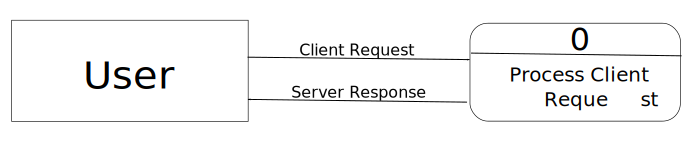
\includegraphics[scale=0.8]{Level0Data}


\section*{Level 1 Data Flow Diagram}

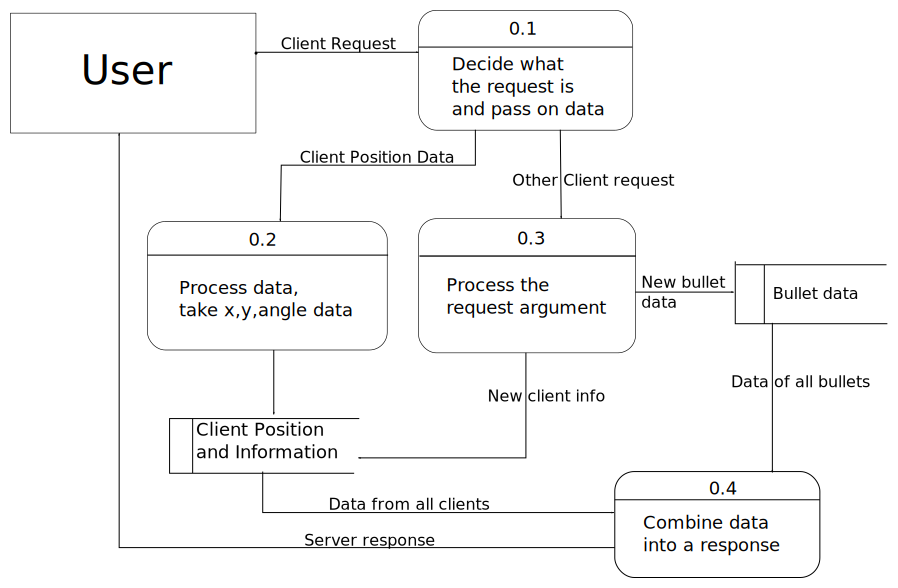
\includegraphics[scale=0.5]{Level1Data}

There is only one entity in my data flow diagram, as information is
both taken from and given to the client. There are to be multiple
clients entities connected to the server at one point, up to 8. The
server will act as a data source, holding data for all connected clients
and sending it to them on request. \\

Data will be stored on the server for user accounts, this will be
a <10MiB database, and on the client side player sprites will be stored
in PNG format for transparency, whilst the maps will likely be stored
in JPG format along with a text file to store map collision data,
i.e. where building are. These sprites could take up between 10 and
20 MiB of data, and the client/server collection will be under 30MiB.
It will be able to be stored on any medium due to this size.\\ 


\subsection{Constraints}


\subsubsection{Hardware}

This is the main constraint of my proposed system as the problem I
am solving is due to low-powered hardware. My solution will have to
run on low-end integrated graphics systems at >30 FPS whilst having
no noticable server lag when running locally to fit with the user's
wants as expressed in the interview. It must also be able to host
the server on both WiFi and Ethernet LAN to cover every possible machine.


\subsubsection{Software}

My proposed system is to be cross-platform, so it must use a programming
language that is also cross-platform as well as any external libraries. 


\subsubsection{Time}

The project must be finished by the deadline, easter 2014.


\subsubsection{User's Knowledge Of Information Technology}

As my user group mainly plays games online, they are familliar with
how to use a program. But to ensure that everyone on all systems can
use my solution, I will keep the program as jargon-free as possible
and as simplistic as I can make it.


\subsubsection{Who will be allowed to use the system?}

The client can be used by anyone, whilst the running server can only
be accessed by the owner of the PC running it. User accounts can only
be accessed by their respective owners, so there will have to be some
way to log in to ensure security.


\subsection{Objectives}


\subsubsection{General Objectives}

My overall objective is to create a fun, multiplayer armoured warfare
game that has depth and end-game content. I want it to run on any
system, regardless of computer specification, whilst making the game
to the users satisfaction.


\subsubsection{Specific Objectives}
\begin{enumerate}
\item By deadline day, my client must be able to communicate across the
network with low latency.
\item By deadline day, it must also be able to run on a low-power PC at
more than 30 Frames Per Second.
\item By deadline day, it must also have user accounts with progression.
\item By deadline day, it must also support up to 8 players.
\item By deadline day, it must also be cross-platform with minimal setup
time.
\item By deadline day, it must be bug-free, being able to run the game without
any crashes.
\end{enumerate}

\subsection{Consideration of Alternative Solutions}
\begin{itemize}
\item I could use an alternative language such as Java as it is in common
use, installed on almost all PCs and is cross platform. This would
fit my specification as the language is compiled, making it run more
effectively on low-end computers. I am also familliar with the language
and how to create games in it, although networking is one of the hardest
features of Java.
\item I could use a WYSIWYG game creator such as gamemaker as it is simple
to use and speeds up production significantly. It is also easy to
learn and has networking extensions to allow for ease of creation. 
\item Alternatively, I could not replace the current system of playing the
game on a low FPS, as it works, albeit barely. 
\end{itemize}

\subsection{Justification of Chosen Solution}

I have chosen to use Python with PyGame for the client and pure Python
for the server, whilst using wxPython for the GUI forms, such as the
server configuration form. This is due to my knowledge of the language
and the ease of networks with inbuilt modules. PyGame also makes game
design more intuitive and efficient, making it able to run on most
any PC. wxPython is a cross-platform GUI toolkit that includes a WYSIWYG
designer and python modules, making the creation of GUI forms simpler.


\section{Design}


\subsection{Overall System Design}

Client Side\\

\includegraphics{\string"ClientFlow - MainClient\string".pdf}\\

Server Side\\

\includegraphics{\string"ClientFlow - ServerSide\string".pdf}\\

Login Server\\

\includegraphics{\string"ClientFlow - Login\string".pdf}


\subsection{Description of Modular Structure of System}

IPSO Table for the proposed system, server-side:\\

\begin{tabular}{|c|c|}
\hline 
Inputs & Processes\tabularnewline
\hline 
\hline 
Username & Sign in player\tabularnewline
\hline 
Password & Search for player in database\tabularnewline
\hline 
Tank Choice & Process the client request\tabularnewline
\hline 
X position & Calculate bullet trajectories\tabularnewline
\hline 
Y position & Calculate if the bullet penetrates\tabularnewline
\hline 
Hull angle & Calculate the HP of hit tanks\tabularnewline
\hline 
Turret angle & Update all connected players\tabularnewline
\hline 
Bullet creation & Update bullet position\tabularnewline
\hline 
Client Request & Calculate angle of bullet impact\tabularnewline
\hline 
Client connection & \tabularnewline
\hline 
\end{tabular}

\begin{tabular}{|c|c|}
\hline 
Outputs & Data Stores\tabularnewline
\hline 
\hline 
Client positions & Client information\tabularnewline
\hline 
Bullet positions & Bullet information\tabularnewline
\hline 
Client HP & User information (stats)\tabularnewline
\hline 
Client XP and progress & \tabularnewline
\hline 
Network response & \tabularnewline
\hline 
Local server information & \tabularnewline
\hline 
\end{tabular}\\


\subsection{Definition of data requirements}

Below are the data dictionaries for each part of my proposed system.

Login database

\begin{tabular}{|c|c|c|c|c|}
\hline 
Field name & Field purpose & Field Type & Example Data & Validation\tabularnewline
\hline 
\hline 
Username & To store the users alias & String & FloatingGhost & Not null\tabularnewline
\hline 
Password & To enable secure login & String/Hashed & 640ab2bae07bedc & Not null\tabularnewline
\hline 
XP & To store the user's progress & Int & 7 & Not null\tabularnewline
\hline 
Tanks & To store the user's unlocked tanks & String & PanzerIV,Maus & Not null\tabularnewline
\hline 
Wins & To store the users number of wins & int & 7 & Not null\tabularnewline
\hline 
\end{tabular}\\

Server variables\\

\begin{tabular}{|c|c|c|c|c|}
\hline 
Field name & Field purpose & Field Type & Example Data & Validation\tabularnewline
\hline 
\hline 
Id & To determine which client is connected & Int & 7 & Not null\tabularnewline
\hline 
x\_pos & To store the clients x position & List of floats & {[}7.7,7.7{]} & Not null\tabularnewline
\hline 
y\_pos & To store the clients y positions & List of floats & {[}7.7,7.7{]} & Not null\tabularnewline
\hline 
angles & To store the clients angles & List of floats & {[}77,77{]} & Not null\tabularnewline
\hline 
turret\_angles & To store the clients turret angles & List of floats & {[}77,77{]} & Not null\tabularnewline
\hline 
\end{tabular}\\

Client variables\\

\begin{tabular}{|c|c|c|c|c|}
\hline 
Field name & Field purpose & Field Type & Example Data & Validation\tabularnewline
\hline 
\hline 
Id & To tell the server who you are & Int & 7 & None\tabularnewline
\hline 
x\_pos & To draw every player on the screen & List of floats & {[}7.7,7.7{]} & None\tabularnewline
\hline 
y\_pos & To draw every player on the screen & List of floats & {[}7,7,7.7{]} & None\tabularnewline
\hline 
angles & To draw every player on the screen & List of floats & {[}77,77{]} & None\tabularnewline
\hline 
turret\_angles & To draw every player on the screen & List of floats & {[}77,77{]} & None\tabularnewline
\hline 
networkComms & To communicate with the server & Custom class & ((``localhost'',9999)) & None\tabularnewline
\hline 
\end{tabular}\\


\subsection{Database Design}


\includegraphics{DatabaseDiag}\\


\subsection{Identification of suitable algorithms}

A large part of my game revolves around armour penetration mechanics,
I.E if the bullet damages the vehicle or not. This is largely dependant
on the bullet's angle of impact to the surface of the tank.
\begin{defn}
Henceforth, \textbf{A.B }shall be used to denote the dot product of
vectors a A and B, where the dot product is defined as

\[
A.B\:=A_{1}B_{1}+A_{2}B_{2}\:=|A||B|cos\theta
\]


Where \textgreek{j} is the angle between the 2 vectors, and |A| is
the modulus or length of the vector given by:

\[
|A|\:=\sqrt{A_{1}^{2}+A_{2}^{2}}
\]


Suppose we have a tank at angle $\alpha_{2}$ and the velocity vector
of the bullet hitting it, with the angle of the velocity vector $\alpha_{1}$,
I.E:

\includegraphics{Collision}

$n$ is the normal to the surface of impact.\end{defn}
\begin{thebibliography}{1}
\bibitem{key-1}NPD Group study into PC Usage: URL: https://www.npd.com/wps/portal/npd/us/news/press-releases/the-npd-group-report-shows-increased-number-of-online-gamers-and-hours-spent-gaming/\end{thebibliography}

\end{document}
